\chapter{The Large Hadron Collider}\label{chapter:lhc}

\section{Introduction}
    The high mass and short life-time of the Higgs Boson ensures that it cannot be readily found in nature.
    In order to study the Higgs Boson then, it must first be artificially created through extremely high-energy physical interactions.
    To achieve this goal, the European Organization for Nuclear Research
        (CERN, from the French \textit{Conseil Européen pour la Recherche Nucléaire})
        set out to build one of the largest and most complex machines in history.
    Construction of this immense device took place over the span of 12 years, from 1995 to 2007.
    The completed project lies in a cavern ranging between 50-175 meters underground, which straddles the French/Swiss border near Geneva, Switzerland.
    This is the Large Hadron Collider, the most powerful particle accelerator ever built.

    \begin{figure}[h]
        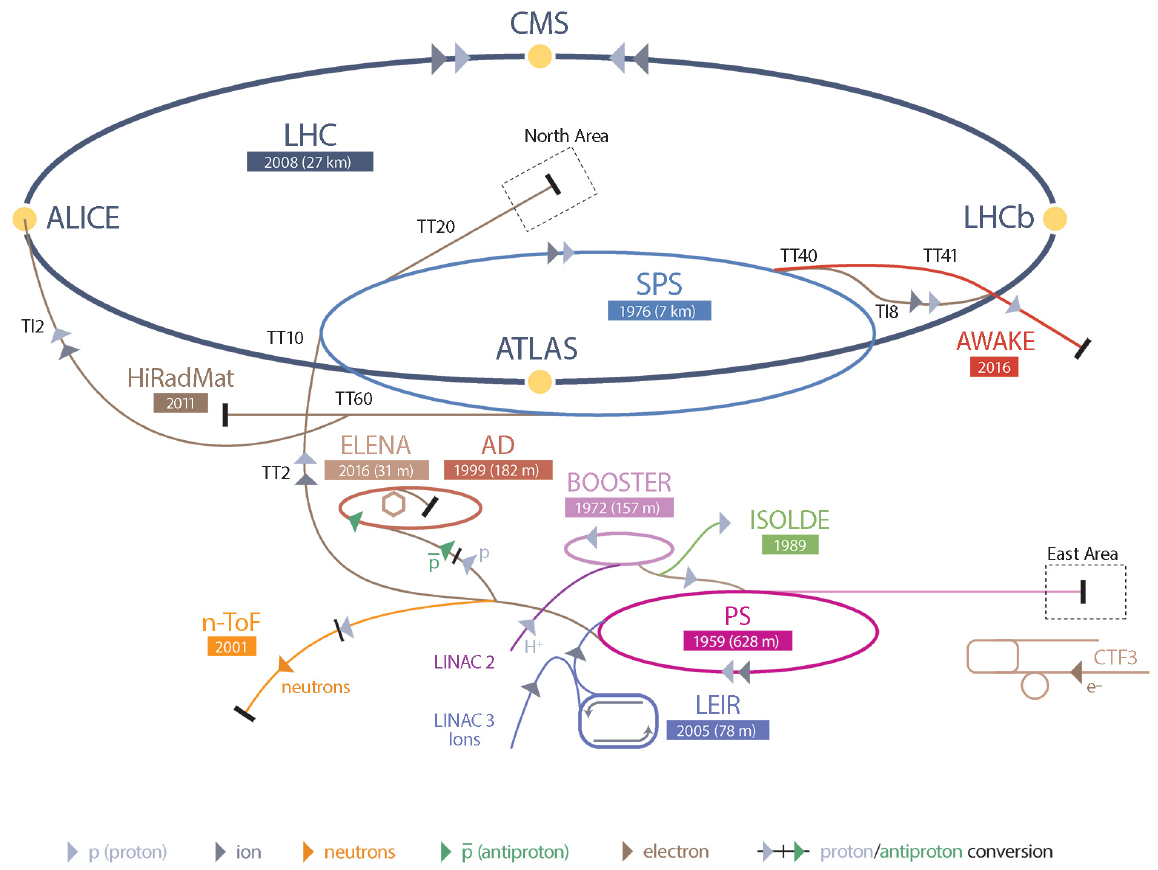
\includegraphics[width=\linewidth,height=\textheight,keepaspectratio]{lhc/lhc_overview}
        \caption{General layout of the LHC, the injection system, and the various detector experiments \cite{lhc_run2}}
        \label{fig:lhc_overview}
    \end{figure}

    A particle accelerator is a machine that uses electromagnetic fields to accelerate charged particles to extremely high energies, with the goal of colliding these particles together.
    The Large Hadron Collider (LHC) is circular in design, with a radius of 26.7 km and a present center of mass (CoM) collision energy of 13 TeV.
    The high CoM energy of the LHC is crucial to its goal, as the cross section of a particle interaction scales with the center of mass energy of the incoming particles.
    At 13 TeV then, the LHC is able to probe physics at energies well beyond that of any previous particle physics experiment.
    Particles are accelerated to such high energies by the particle injection system and the main accelerator ring.
    The subsequent collision of those particles is then handled at ``Interaction Points,'' in which the accelerated particles are intentionally diverted into each other.
    Understanding how the LHC carries out these functions is critical to understanding the physics interactions it produces.


\section{Accelerator Ring}
    The most basic function of a particle accelerator is to accelerate particles to high energies.
    Particle acceleration is performed using electromagnetic fields to push and pull charged particles along the path of the accelerator.
    The earliest accelerator experiments operated in what is known as a fixed-target arrangement, in which a single beam of particles is accelerated into a stationary wall of material.
    Such collisions have interaction energies that go as $\approx \sqrt{2 E \times m c^2}$ for a high energy ($E$) particle colliding with a stationary particle of mass $m$.
    The LHC, like many modern accelerators, instead uses two independent particle beams which are collided with each other.
    Due to the properties of Lorentz transformations, these dual-beam colliders achieve much higher CoM energies of $\approx 2 \sqrt{E_1 E_2}$ \cite{modern_and_future_colliders}.
    Aside from the target arrangement, there are a variety of design shapes accelerators can take, from linear accelerators to synchrotrons to circular accelerators and more.
    The LHC falls into the latter most category as a circular collider.

    Circular accelerators operate by moving charged ions through a series of Radio Frequency (RF) cavities, arranged along the accelerator ring, which generate electric fields oscillating at high-frequencies.
    Their primary advantage is that they are able to accelerate ions repeatedly through the same electric fields, allowing for much higher energies within a smaller volume.
    However, directing charged ions in a circular path comes at the cost of both radiative energy loss and a critical dependence on size and magnetic field strength.
    The issue of energy loss arises from the fact that charged particles lose energy while accelerating, in the form of synchrotron radiation.
    Power loss from synchrotron radiation $P_\gamma$ scales proportional to a particle's energy $E$, mass $m$, and bending radius $r$ as $P_\gamma \propto \frac{E^4}{m^4 r^2}$ \cite{2007_Book_ParticleAcceleratorPhysics}.
    The LHC is able to mitigate this issue primarily through its use of protons as the colliding medium.
    Due to their high mass, the energy losses protons incur from synchrotron radiation are quartically suppressed and thus easily overcome (7 keV losses at the 6.5 TeV operating point of the LHC \cite{lhc_machine}). % table 4.1

    The more challenging aspect of a circular collider is that keeping a charged particle moving along a curved path requires constant deflection from a magnetic field.
    This requirement places a hard upper bound on the energy any collider can achieve.
    Relating the Lorentz force to the formula for centripetal acceleration, one can find the magnetic field $B$ needed to bend a relativistic particle as $B=\frac{E/c}{q r}$.
    Rearranging for energy, $E = q B c r$, shows that the maximum energy a circular accelerator can achieve is fundamentally limited by the product of the magnetic field strength $B$ and the radius of the accelerator $r$.
    Using leading-edge superconducting electromagnets, the LHC can achieve a field strength of around 8 Tesla.
    Even with magnets of this strength though, the earlier formula puts an absolute lower bound on the accelerator's radius at 2.7 km.
    Of course, practical considerations (e.g.\ the magnetic field cannot realistically be present continuously throughout the entire accelerator tunnel) shift that radius even higher, to the actual radius of 26.7 km.
    This giant primary ring is actually not the only accelerator used by the LHC however.
    The full acceleration process is handled by a sequence of accelerators, constituting the LHC injection system.

    Particles cannot be simply dropped directly into the main accelerator ring and accelerated from a standstill.
    Instead, they must be injected into the main ring already at relativistic speeds.
    The LHC Injection System consists of a series of smaller particle accelerators that take initially stationary hydrogen atoms and drive them to energies usable by the main ring.
    From a standstill, hydrogen ions are accelerated to 50 MeV by Linac2, in groups of billions of protons called ``bunches" \cite{lhc_run2}.
    From Linac2, the roughly 2800 bunches are subsequently boosted to 1.4 GeV, 25 GeV, and then 450 GeV by the Proton Synchrotron Booster (PSB), Proton Synchrotron (PS), and Super Proton Synchrotron (SPS) respectively (see figure \ref{fig:lhc_overview}).
    After the SPS, they are injected into the main LHC ring where they are accelerated to their final energy of 6.5 TeV \cite{lhc_machine}.
    With the LHC's proton beams accelerated to their operating point, it is able to collide them together for a record-setting 13 TeV center-of-mass interaction energy.


\section{Interaction Region} \label{sec:lhc-interaction_region}
    The LHC accelerates particles to truly phenomenal energies, but it does so only for the purpose of bringing them to a very abrupt and cataclysmic stop.
    These particle collisions are only able to take place at a few specific points along the main ring where the particle beams are diverted into each other.
    The technical details of how particles are redirected into these Interaction Points is non-trivial, but is also not of critical importance to the subject of this thesis.
    What matters for this thesis is not the ``how" of collision, but rather the question of ``how often".

    \begin{figure}[h]
        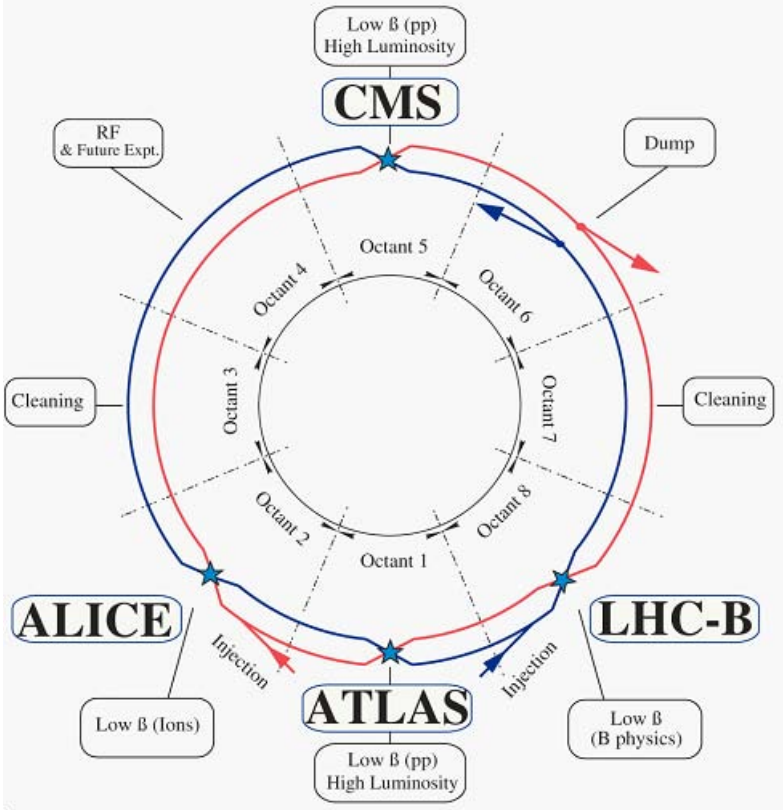
\includegraphics[width=\linewidth,height=\textheight,keepaspectratio]{lhc/interaction_points}
        \caption{Map of the LHC's various interaction points \cite{lhc_machine}}
        \label{fig:interaction_points}
    \end{figure}

    \FloatBarrier

    How often exotic events are produced is critically important to hypothesis testing in physics.
    Indeed, the rate an event is observed to occur at the LHC is the entire basis for the dismissal or success of particle physics hypotheses, as will be discussed in more detail in later chapters.
    Examining how this rate is determined, and the role the LHC plays in it, is therefore of utmost importance.
    The frequency with which some kind of particle interaction occurs at the LHC is a probabilistic event, determined by a number of factors.
    As an analogy, imagine somebody repeatedly throwing a ball at a window on the wall of a barn.
    For a given throw, there is some probability that the ball will hit the window, calculated as the ratio of the area of the window to the total area the thrower could possibly hit.
    Provided that the person throws the ball with some given frequency, there is then a probability of the ball hitting the window per unit time.
    Over some period of time, this would yield some expected total number of successful hits.

    \begin{table} \centering
\begin{tabular}{|l|l|l|l|}
\hline
Year & Dataset                              & \multicolumn{2}{c|}{Integrated Luminosity}  \\
\hline
     &                                      & Delivered    & Recorded    \\
\hline
2015 & pp @ $\sqrt{s} = 13$ TeV (50 ns)     &  102.2  pb\textsuperscript{-1}   & 94.5  pb\textsuperscript{-1}  \\
     & pp @ $\sqrt{s} = 13$ TeV (25 ns)     &  3.88   fb\textsuperscript{-1}   & 3.63  fb\textsuperscript{-1}  \\
     & pp @ $\sqrt{s} = 5.02$ TeV           &  26.1   pb\textsuperscript{-1}   & 25.6  pb\textsuperscript{-1}  \\
     & Pb-Pb @ $\sqrt{s_{NN}} = 5.02$ TeV   &  0.51   nb\textsuperscript{-1}   &  0.50 nb\textsuperscript{-1}  \\
\hline
2016 & pp @ $\sqrt{s} = 13$ TeV             &  38.0   fb\textsuperscript{-1}   & 35.5  fb\textsuperscript{-1}  \\
     & p-Pb @ $\sqrt{s_{NN}} = 8.16$ TeV    &  170    nb\textsuperscript{-1}   & 167   nb\textsuperscript{-1}  \\
     & p-Pb @ $\sqrt{s_{NN}} = 5.02$ TeV    &  0.44   nb\textsuperscript{-1}   &  0.43 nb\textsuperscript{-1}  \\
\hline
2017 & pp @ $\sqrt{s} = 13$ TeV             &  49.0   fb\textsuperscript{-1}   & 46.4  fb\textsuperscript{-1}  \\
     & Xe-Xe @ $\sqrt{s_{NN}} = 5.44$ TeV   &  1.97   nb\textsuperscript{-1}   &  1.96 nb\textsuperscript{-1}  \\
     & pp @ s = 5.02 TeV ($\mu=2$)          &  273    pb\textsuperscript{-1}   & 270   pb\textsuperscript{-1}  \\
     & pp @ $\sqrt{s} = 13$ TeV ($\mu=2$)   &  150    pb\textsuperscript{-1}   & 148   pb\textsuperscript{-1}  \\
\hline
2018 & pp @ $\sqrt{s} = 13$ TeV             &  62.1   fb\textsuperscript{-1}   & 60.0  fb\textsuperscript{-1}  \\
     & pp @ $\sqrt{s} = 13$ TeV ($\mu=2$)   &  213    pb\textsuperscript{-1}   & 208   pb\textsuperscript{-1}  \\
     & Pb-Pb @ $\sqrt{s_{NN}} = 5.02$ TeV   &  1.78   nb\textsuperscript{-1}   &  1.74 nb\textsuperscript{-1}  \\ 
\hline
\end{tabular}
\caption{
    Integrated Luminosity per Run at ATLAS \cite{data_quality}
    The (25/50 ns) after some datasets for 2015 refer to the bunch spacing for that run.
    The ($\mu=2$) in 2017 and 2018 refer to the the pile up of that run.
}
\label{tab:dataset_lum}

\end{table}


    Hitting the window with a ball is analogous to particles in a particle accelerator interacting to produce some specific physics process.
    The area of the window corresponds to the physics process's \textit{cross-section}, which is measured using a unit of area called a ``barn" (1 b = $10^{-28}$ m\textsuperscript{2}, pun very much intended).
    Meanwhile, the other components comprising the probability of a hit per unit time
        -- the total area which can be hit and the frequency of throws --
        are all collected together into a single quantity called \textit{luminosity} (measured in units of $b^{-1}t^{-1}$). 
    The probability of a physics process occurring per unit time is then obtained by multiplying luminosity with the process's cross-section.
    As noted earlier, the cross-section of an event scales with the center-of-mass energy of the interaction,
        hence the drive for ever-more powerful colliders.
    For reference, even at the LHC's 13 TeV CoM energy,
        the \vbfhhproc process used in this thesis still only has a SM (all $\kappa$-values equal to 1) cross-section of 1.18 fb (femto-barns).
    This is astonishingly small.
    Even if the metaphorical barn window were reduced to a single silicon atomic nucleus,
        its cross-section ($\approx 4 \times 10^{23}$ \ifb)
        would still be 400 billion \textit{trillion} times larger than that of the VBF di-Higgs process.
    Producing any significant number of these events thus neccesitates maximizing the LHC's integrated luminosity.

    Luminosity can be improved by increasing the particle interaction rate through a number of methods.
    Continuing the analogy of the ball and barn, an obvious improvement would be to improve the thrower's aim.
    At the LHC, this corresponds to tightening the particle beam width by increasing the power of the quadrupole focusing magnets.
    One could also throw balls at a faster rate.
    More balls per second means more chances of a hit per second.
    The same can be done at the LHC by decreasing the bunch-spacing, the time between bunch-crossings.
    Along the same lines, the thrower could throw more balls at the window at a time,
        equivalent in the accelerator situation to increasing the number of bunches in circulation around the ring
        (or increasing the protons per bunch).
    Finally, the overall number of collisions can be steadily increased by extending the time the machine is running, analogous to having the thrower keep throwing balls for a longer time.
    All of these specifications -- beam-spot, bunch-spacing, bunch size, and runtime -- are planned to be varied over the lifetime of the LHC in different operating configurations.
    
    \begin{table}[tbh]
   \begin{center}
       \caption{Theoretical event yields.
                Results retrieved via pyAMI tool~\cite{pyAMIdoc}\cite{hh4b_2021_int_note}.
             }
       \label{tab:mcyields}
       \footnotesize
       \begin{tabular}{|lll|r|r|}
       \hline
           \kl & \kvv & \kv & {AMI $\sigma$ [fb]} & Event Yield  \\
               &      &     &                     & (for 126 fb\textsuperscript{-1}) \\       
           \hline
           1  & 1   & 1    &	 1.18 &  149.13 \\
           1  & 0   & 1    &	18.59 & 2342.71 \\
           1  & 0.5 & 1    &	 6.62 &  833.83 \\
           1  & 1.5 & 1    &	 2.30 &  290.20 \\
           1  & 2   & 1    &	 9.97 & 1256.55 \\
           1  & 3   & 1    &	44.94 & 5662.94 \\
           0  & 1   & 1    &	 3.17 &  398.90 \\
           2  & 1   & 1    &	 1.07 &  134.57 \\
           10 & 1   & 1    &	67.38 & 8489.50 \\
           1  & 1   & 0.5  &	 7.53 &  948.64 \\
           1  & 1   & 1.5  &	45.41 & 5721.91 \\
           0  & 0   & 1    &	25.40 & 3200.40 \\
           -5 & 1   & 0.5  &	 4.45 &  560.84 \\
       \hline
       \end{tabular}
   \end{center}
\end{table}


    So far, there have been two complete ``Runs" of the LHC, with the data from those runs further subdivided by year and operational configuration.
    The data used in this thesis comes from Run 2 data using proton-proton collisions at a CoM energy of 13 TeV.
    For most of Run 2, the bunch spacing was 25 ns between bunches, though early periods (not used in this analysis) operated at a lower 50 ns bunch spacing.
    The beam spot in the main ring is XXX $\mu$m, but varies at the different interaction regions in which the beams collide.
    The relevant interaction region for this discussion is Interaction Region 1 (IR1, see Fig. \ref{fig:interaction_points}), the location of the ATLAS detector.
    Here, the particle beam width is focused to 80 cm using several powerful quadrupole magnets.
    Total runtime, as far as data is concerned, is not measured as simply the time the machine has been running, but rather the time spent collecting data.
    Data-taking takes place between the time ``stable beams" are declared by the LHC, until enough protons have been depleted from the ring that it needs to undergo another bunch injection and acceleration process.
    This time frame is known as a \textit{fill},
        and is itself further subdivided into smaller \textasciitilde 60 second time frames called \textit{luminosity blocks},
        periods of data taking in which luminosity is relatively stable \cite{data_quality}.
    These various parameters taken together over the four year period of Run 2 produce the total integrated luminosity of data available for observation (see Table \ref{tab:dataset_lum} ).
    Due to occasional issues during data collection, some data is deemed unusable,
        bringing the total available integrated luminosity for this process to 126 fb\textsuperscript{-1}.
    Table \ref{tab:mcyields} shows the number of \vbfhhproc events expected to be produced by the LHC at IR1,
        for various possible coupling arrangements.
    The actual process of observing and recording this data however, is a massive undertaking all its own, and is carried out by ATLAS.
